% Figure 1: how a scene is classified by the pruned network (top) and the PMP schedule (bottom). TikZ; no data in this figure.
\begin{tikzpicture}[
    font=\footnotesize,
    box/.style={draw, rounded corners=1.5pt, minimum height=0.7cm, align=center, inner sep=2.5pt, line width=0.5pt},
    prune/.style={box, fill=red!10, draw=red!60!black},
    train/.style={box, fill=blue!8, draw=blue!50!black},
    base/.style={box, fill=gray!12, draw=gray!70!black},
    keep/.style={box, fill=green!12, draw=green!45!black},
    arr/.style={-{Stealth[length=4.5pt]}, line width=0.6pt},
    bar/.style={draw=blue!60!black, fill=blue!35, line width=0.3pt},
    cut/.style={draw=red!70!black, fill=white, dash pattern=on 1pt off 0.8pt, line width=0.35pt}
]
  % ---- (a) one scene through the pruned network -------------------------------------------------------
  \node[anchor=west, font=\footnotesize\bfseries] at (-0.7,1.25) {(a) An image becomes a label};
  \node[inner sep=0pt, draw, line width=0.4pt] at (-0.58,0) {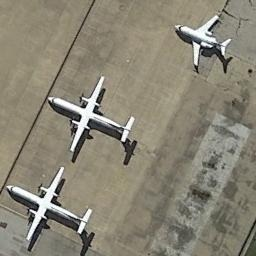
\includegraphics[width=1.05cm,height=1.05cm]{img_aerial.jpg}};
  \node[inner sep=0pt, draw, line width=0.4pt] at (0.58,0) {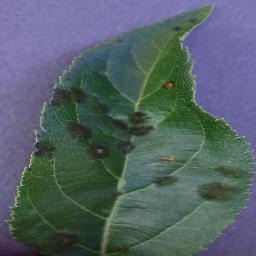
\includegraphics[width=1.05cm,height=1.05cm]{img_leaf.jpg}};
  \node[align=center, font=\scriptsize] at (0,-1.15) {input images: aerial\\scene, leaf photo\\(13-band patches too)};
  \foreach \cx/\pat in {2.3/{0/1,1/1,2/1,3/0,4/1,5/1}, 3.6/{0/1,1/0,2/1,3/1,4/0,5/1}, 4.9/{0/0,1/1,2/0,3/1,4/0,5/1}, 6.2/{0/0,1/0,2/1,3/0,4/0,5/1}} {
    \draw[rounded corners=1.5pt, fill=white, line width=0.5pt] (\cx-0.5,-0.62) rectangle (\cx+0.5,0.62);
    \foreach \j/\k in \pat {
      \ifnum\k=1 \draw[bar] ({\cx-0.38+0.15*\j},-0.4) rectangle ++(0.08,0.8);
      \else \draw[cut] ({\cx-0.38+0.15*\j},-0.4) rectangle ++(0.08,0.8); \fi
    }
  }
  \foreach \x in {2.8,4.1,5.4} \draw[arr] (\x,0) -- ++(0.3,0);
  \draw[arr] (1.2,0) -- (1.77,0);
  \node[text width=5.8cm, align=center, font=\scriptsize] at (4.25,-1.3) {ImageNet-pretrained trunk (ResNet-18 or MobileNetV2): the inner channels of each block are scored and the lowest scorers (dashed) are removed; deeper blocks lose more};
  \node[train, minimum width=1.9cm] (pool) at (8.55,0) {global average\\pool, L2 norm};
  \draw[arr] (6.7,0) -- (pool.west);
  \foreach \i/\v in {0/15,1/60,2/30,3/80,4/20,5/55,6/40,7/70} \fill[blue!\v] ({10.0+0.15*\i},-0.17) rectangle ++(0.13,0.34);
  \node[font=\scriptsize] at (10.55,0.42) {embedding};
  \draw[arr] (pool.east) -- (9.93,0);
  \node[keep, minimum width=2.1cm] (cos) at (12.45,0) {cosine similarity\\to 5 prototypes};
  \draw[arr] (11.25,0) -- (cos.west);
  \node[base, minimum width=1.3cm] (out) at (14.75,0) {label =\\nearest};
  \draw[arr] (cos.east) -- (out.west);
  \node[base, minimum width=2.9cm] (sup) at (12.45,-1.55) {$K$ support scenes per class:\\mean embedding = prototype};
  \draw[arr] (sup.north) -- (cos.south);
  % ---- (b) the PMP schedule -----------------------------------------------------------------------------
  \node[anchor=west, font=\footnotesize\bfseries] at (-0.7,-2.55) {(b) The PMP schedule};
  \node[base] (s0) at (0.45,-3.45) {ImageNet\\weights};
  \node[train, right=0.28cm of s0] (ce) {S0: CE on\\base classes};
  \node[prune, right=0.28cm of ce] (p1) {P1: prune\\to 60\%};
  \node[train, right=0.28cm of p1] (r1) {R: recover\\with CE};
  \node[train, right=0.28cm of r1] (m) {M: 1000\\episodes};
  \node[prune, right=0.28cm of m] (p2) {P2: prune\\to budget};
  \node[train, right=0.28cm of p2] (r2) {R: recover\\with CE};
  \foreach \a/\b in {s0/ce, ce/p1, p1/r1, r1/m, m/p2, p2/r2} \draw[arr] (\a) -- (\b);
  \node[box, dashed, draw=red!60!black, below=0.5cm of p2, font=\scriptsize] (g) {$G_{\mathrm{meta}}$: filter-gradient\\norm collected in M};
  \draw[arr, dashed, red!60!black] (m.south) |- (g.west);
  \draw[arr, dashed, red!60!black] (g.north) -- (p2.south);
  \node[right=0.4cm of r2, align=left, font=\scriptsize] {\textcolor{blue!50!black}{$\blacksquare$} training\\\textcolor{red!60!black}{$\blacksquare$} pruning};
\end{tikzpicture}
